\section{Kết quả}
\label{sec:results}

Mọi số liệu trong mục này được đọc từ các tệp kết quả do chương trình ghi ra (\texttt{results/final}, \texttt{results/tuning}, \texttt{results/baselines}); không có con số nào nhập tay. Cấu hình của từng mô hình là cấu hình tốt nhất trên validation (\cref{tab:tuning}); mỗi mô hình được huấn luyện lại một lần trên $50\,000$ ảnh train rồi mới chạm vào tập test.

\subsection{Siêu tham số được chọn}
\begin{table}[H]
\centering\small
\begin{tabular}{@{}lp{9.0cm}r@{}}
\toprule
Mô hình & Siêu tham số được chọn & Số cấu hình đã chạy \\
\midrule
Gaussian NB & \texttt{var\_smoothing=0.1} & 12 \\
Softmax regression & \texttt{learning\_rate=0.03, l2=0.0, epochs=67, batch\_size=128} & 16 \\
MLP & \texttt{hidden\_sizes=(512, 256), learning\_rate=0.05, momentum=0.9, p\_drop=0.0, batch\_size=128, epochs=40} & 22 \\
AdaBoost-SAMME & \texttt{n\_estimators=393, max\_depth=10, learning\_rate=0.1, n\_bins=32, max\_features=0.5} & 14 \\
\bottomrule
\end{tabular}

\caption{Cấu hình chọn bằng validation. \texttt{epochs} của softmax và \texttt{n\_estimators} của AdaBoost lấy từ đường cong validation của một lần chạy dài (tối đa 100 epoch và 400 vòng).}
\label{tab:tuning}
\end{table}

\Cref{tab:sweeps} tóm tắt từng lượt quét: khoảng dao động của validation cho thấy tham số nào thật sự quan trọng. Độ sâu cây quyết định (AdaBoost) và kích thước/hình dạng mạng (MLP) là hai tham số kéo độ chính xác nhiều nhất; với Naïve Bayes, \texttt{var\_smoothing} mặc định $10^{-9}$ cho kết quả rất tệ (xem \cref{sec:discussion}).

\begin{table}[H]
\centering\footnotesize\setlength{\tabcolsep}{3.5pt}
\begin{tabular}{llrrrl}
\toprule
Mô hình & Siêu tham số & Số giá trị & Val thấp nhất & Val cao nhất & Giá trị tốt nhất \\
\midrule
Gaussian NB & \texttt{var\_smoothing} & 12 & 56.05 & 79.67 & \texttt{0.1} \\
Softmax regression & \texttt{learning\_rate} & 6 & 88.03 & 91.72 & \texttt{0.03} \\
Softmax regression & \texttt{batch\_size} & 6 & 90.23 & 91.72 & \texttt{128} \\
Softmax regression & \texttt{l2} & 5 & 91.20 & 91.76 & \texttt{0.0} \\
MLP & \texttt{hidden\_sizes} & 8 & 95.65 & 98.18 & \texttt{(512, 256)} \\
MLP & \texttt{learning\_rate} & 5 & 96.41 & 98.18 & \texttt{0.05} \\
MLP & \texttt{momentum} & 4 & 97.49 & 98.18 & \texttt{0.9} \\
MLP & \texttt{batch\_size} & 4 & 95.57 & 98.18 & \texttt{128} \\
MLP & \texttt{p\_drop} & 5 & 97.79 & 98.18 & \texttt{0.0} \\
AdaBoost-SAMME & \texttt{max\_depth} & 5 & 77.23 & 95.98 & \texttt{10} \\
AdaBoost-SAMME & \texttt{max\_features} & 3 & 95.98 & 96.29 & \texttt{0.5} \\
AdaBoost-SAMME & \texttt{learning\_rate} & 4 & 96.29 & 97.02 & \texttt{0.1} \\
AdaBoost-SAMME & \texttt{n\_bins} & 4 & 96.73 & 97.02 & \texttt{32} \\
CNN & \texttt{channels} & 3 & 97.29 & 97.84 & \texttt{(16, 32)} \\
CNN & \texttt{kernel\_size} & 2 & 97.29 & 97.84 & \texttt{3} \\
CNN & \texttt{dense} & 2 & 97.84 & 98.57 & \texttt{(64)} \\
CNN & \texttt{learning\_rate} & 3 & 11.24 & 98.61 & \texttt{0.01} \\
CNN & \texttt{batch\_size} & 3 & 98.28 & 98.61 & \texttt{128} \\
CNN & \texttt{p\_drop} & 2 & 98.61 & 98.65 & \texttt{0.2} \\
\bottomrule
\end{tabular}

\caption{Từng lượt quét siêu tham số trên tập validation (độ chính xác, \%). Các lượt quét chạy tuần tự nên mỗi bảng ứng với phần còn lại giữ ở giá trị tốt nhất đã tìm được trước đó.}
\label{tab:sweeps}
\end{table}

\Cref{fig:sweep-mlp} cho thấy các lượt quét của MLP, kèm khoảng cách giữa train và validation. Hình của ba mô hình còn lại nằm ở \cref{app:sweeps}. Các thanh thời gian ở dải dưới chỉ mang tính tham khảo: một số lượt quét có thể chạy cùng lúc với công việc khác trên máy nên thời gian không so sánh được tuyệt đối với bảng thời gian cuối.

\begin{figure}[H]
\centering
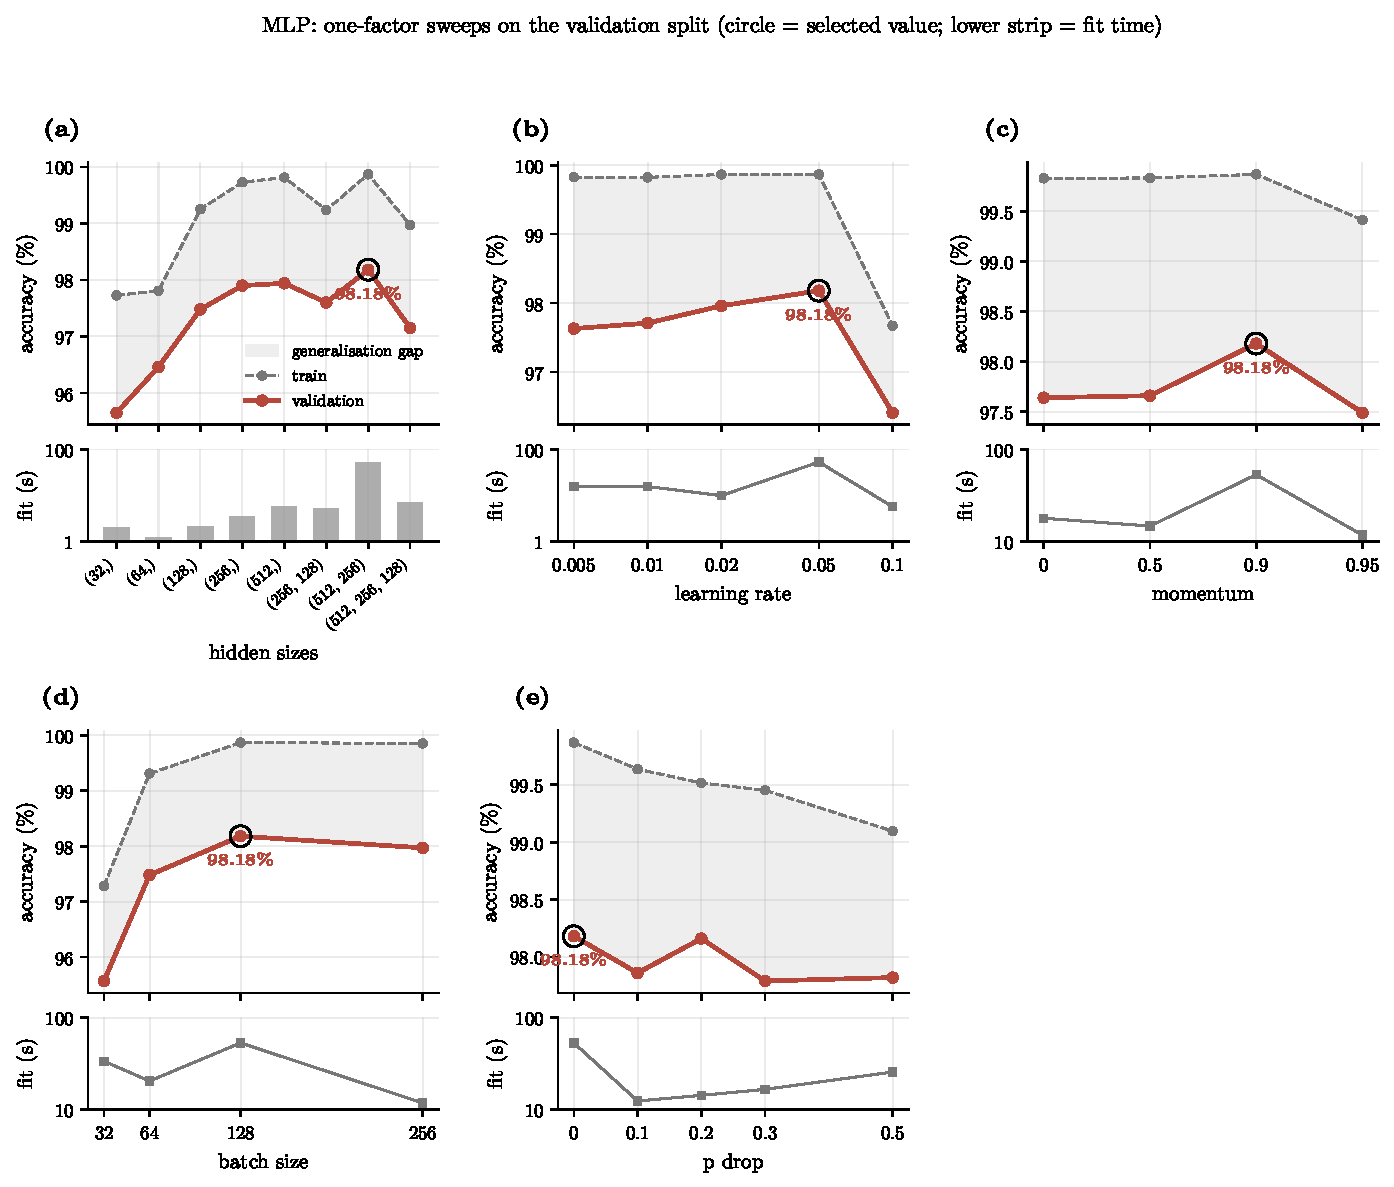
\includegraphics[width=0.96\textwidth]{../results/figures/sweep_mlp.pdf}
\caption{MLP: quét từng siêu tham số trên validation. Vòng tròn đánh dấu giá trị được chọn.}
\label{fig:sweep-mlp}
\end{figure}

\subsection{Độ chính xác và các độ đo}
\begin{table}[H]
\centering\small
\begin{tabular}{lrrrrrr}
\toprule
Mô hình & Train & Val & Test & P$_{\text{macro}}$ & R$_{\text{macro}}$ & F1$_{\text{macro}}$ \\
\midrule
Gaussian NB & 80.13 & 79.67 & \textbf{81.32} & 82.98 & 80.95 & 81.16 \\
Softmax regression & 93.62 & 92.15 & \textbf{92.52} & 92.45 & 92.41 & 92.42 \\
MLP & 99.87 & 98.18 & \textbf{98.24} & 98.23 & 98.23 & 98.23 \\
AdaBoost-SAMME & 100.00 & 97.59 & \textbf{97.60} & 97.58 & 97.58 & 97.58 \\
CNN & 99.40 & 98.65 & \textbf{98.80} & 98.79 & 98.79 & 98.79 \\
\bottomrule
\end{tabular}

\caption{Độ chính xác (\%) trên train, validation, test và precision/recall/F1 macro trên test. Một seed (42) cho mỗi mô hình.}
\label{tab:accuracy}
\end{table}

Độ chính xác test của bốn mô hình là \accTestNB, \accTestSM, \accTestMLP{} và \accTestADA\% (\cref{tab:accuracy}). Với $n=10\,000$ ảnh, khoảng tin cậy nhị thức $95\%$ cho độ chính xác quanh $98\%$ rộng khoảng $\pm0.3$ điểm phần trăm, nên chênh lệch giữa MLP và AdaBoost (\accTestMLP\% so với \accTestADA\%) không nhỏ hơn nhiễu lấy mẫu một cách hiển nhiên. Vì cả hai được đánh giá trên cùng ảnh nên chúng tôi dùng kiểm định McNemar chính xác: có \mcOnlyMLP{} ảnh chỉ MLP đoán đúng và \mcOnlyADA{} ảnh chỉ AdaBoost đoán đúng, $p=$ \mcP. Kết luận này chỉ nói về một seed và một phép chia dữ liệu.

\begin{figure}[H]
\centering
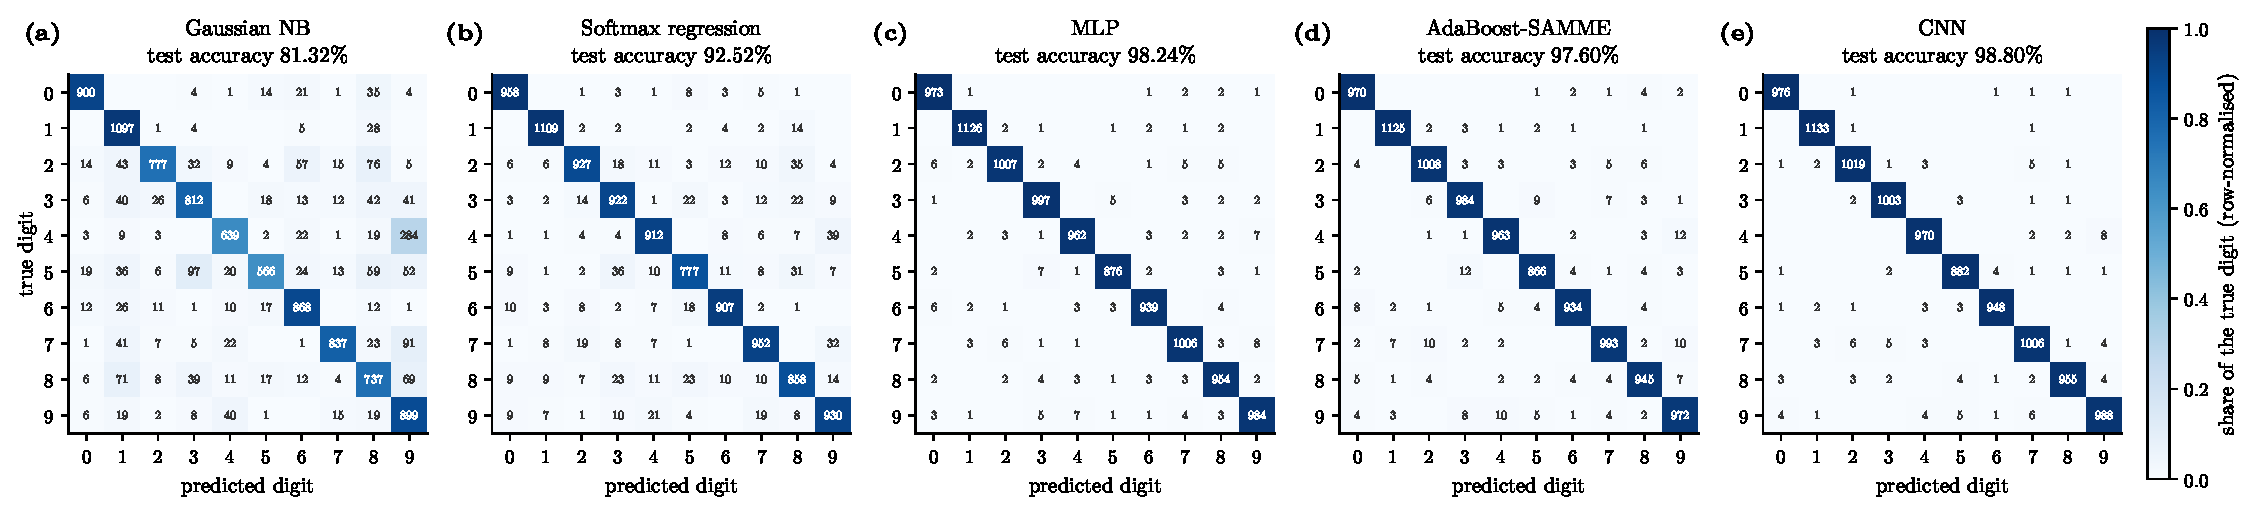
\includegraphics[width=\textwidth]{../results/figures/confusion_all.pdf}
\caption{Ma trận nhầm lẫn trên tập test (hàng = chữ số thật, chuẩn hóa theo hàng; số trong ô là số ảnh).}
\label{fig:confusion}
\end{figure}

\subsection{Thời gian}
\begin{table}[H]
\centering\small
\begin{tabular}{lrrr}
\toprule
Mô hình & Huấn luyện (s) & Dự đoán 10\,000 mẫu (s) & 1 mẫu (ms) \\
\midrule
Gaussian NB & 0.4 & 0.226 & 0.076 \\
Softmax regression & 12.7 & 0.024 & 0.010 \\
MLP & 11.0 & 0.051 & 0.042 \\
AdaBoost-SAMME & 817.9 & 0.751 & 18.705 \\
CNN & 143.0 & 1.163 & 0.315 \\
\bottomrule
\end{tabular}

\caption{Thời gian trên CPU (cấu hình máy ở \cref{sec:hardware}). Huấn luyện trên $50\,000$ ảnh; dự đoán $10\,000$ ảnh test; độ trễ là trung vị của 200 lần dự đoán một ảnh.}
\label{tab:time}
\end{table}

\begin{figure}[H]
\centering
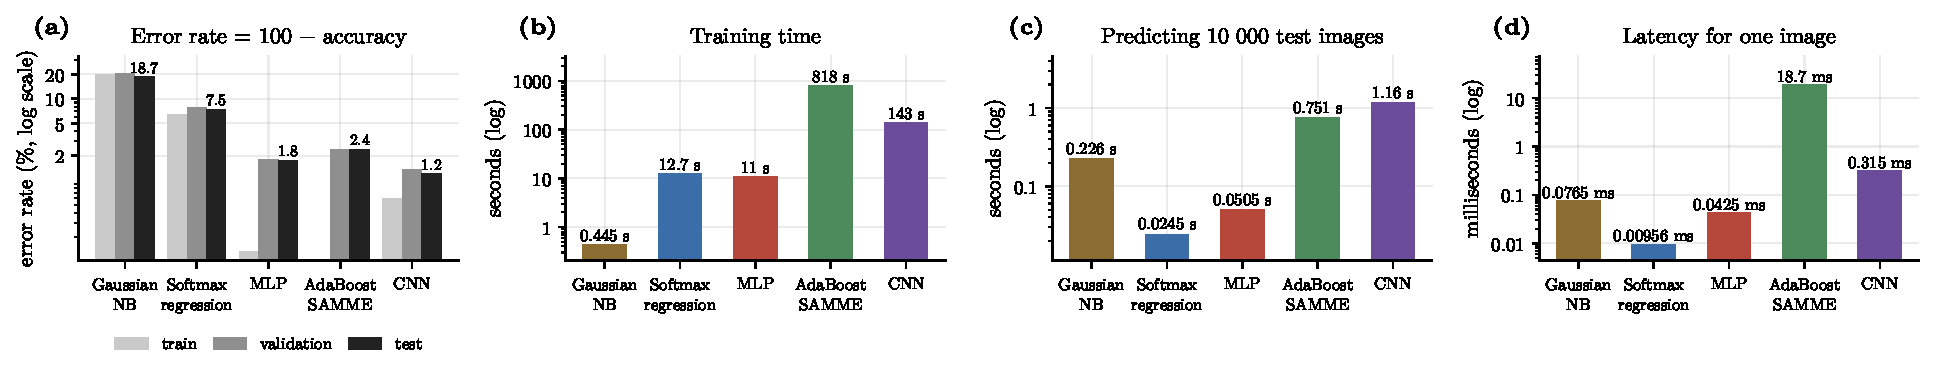
\includegraphics[width=\textwidth]{../results/figures/benchmark.pdf}
\caption{Lỗi và thời gian của bốn mô hình, thang log. Vạch sáng/trung/đậm trong (a) là train/validation/test; sai số train của AdaBoost bằng 0 nên cột train không hiện trên thang log.}
\label{fig:benchmark}
\end{figure}

\subsection{So sánh công bằng với scikit-learn}
Với mỗi mô hình, scikit-learn được dùng \emph{cùng siêu tham số} đã chọn ở trên, huấn luyện trên cùng $50\,000$ ảnh và đánh giá trên cùng tập test (không chọn lại siêu tham số cho scikit-learn). Đây là so sánh về tính đúng đắn của cài đặt hơn là cuộc đua về thuật toán.

\begin{table}[H]
\centering\small
\begin{tabular}{lrrrrr}
\toprule
Mô hình & Test (ours) & Test (sklearn) & $|\Delta|$ & Fit ours (s) & Fit sklearn (s) \\
\midrule
Gaussian NB & 81.32 & 81.32 & 0.00 & 0.4 & 0.2 \\
Softmax regression & 92.52 & 91.86 & 0.66 & 12.7 & 154.6 \\
MLP & 98.24 & 98.02 & 0.22 & 11.0 & 57.8 \\
AdaBoost-SAMME & 97.60 & 97.50 & 0.10 & 817.9 & 1892.8 \\
\bottomrule
\end{tabular}

\caption{Bản tự cài đặt so với scikit-learn trên tập test (độ chính xác, \%) và thời gian huấn luyện.}
\label{tab:sklearn}
\end{table}

\begin{itemize}
\item \textbf{Naïve Bayes} trùng khớp hoàn toàn (\accTestNB\% cả hai), đúng như kiểm thử số học ở Mục~\ref{sec:verification}.
\item \textbf{Softmax}: bản của chúng tôi cao hơn \diffSkSM{} điểm phần trăm. Đây không phải lợi thế thuật toán: scikit-learn chạy L-BFGS đến giới hạn 1000 vòng (cảnh báo chưa hội tụ), không dừng sớm và không chính quy hóa ($\ell_2=0$ như cấu hình được chọn), còn chúng tôi dừng ở epoch được chọn trên validation.
\item \textbf{MLP}: \accTestMLP\% so với \accTestSkMLP\%. Cùng kiến trúc, momentum, batch và quy tắc dừng sớm, nhưng khởi tạo, thứ tự lấy mẫu và cách tách tập dừng sớm khác nhau nên chênh \diffSkMLP{} điểm phần trăm nằm trong dao động giữa các seed (xem \cref{tab:augmentation-mlp}).
\item \textbf{AdaBoost}: \accTestADA\% so với \accTestSkADA\% (chênh \diffSkADA). Hai bản không cùng thuật toán chia: của chúng tôi dùng histogram \texttt{n\_bins}=32 và chọn ngẫu nhiên một nửa số đặc trưng cho mỗi cây, scikit-learn tìm ngưỡng chính xác trên mọi đặc trưng. Thời gian huấn luyện (\fitADA\,s so với \fitSkADA\,s) vì vậy không phải so sánh sạch, và lượt chạy scikit-learn có trùng thời gian với một thí nghiệm khác trên cùng máy.
\end{itemize}
Thời gian của các bản scikit-learn khác nhau chủ yếu do thư viện đại số tuyến tính và cách cài đặt (ví dụ \texttt{lbfgs} lặp 1000 vòng trên toàn bộ dữ liệu), không nên đọc thành nhận xét về thuật toán.

\subsection{Đường cong học}
\begin{figure}[H]
\centering
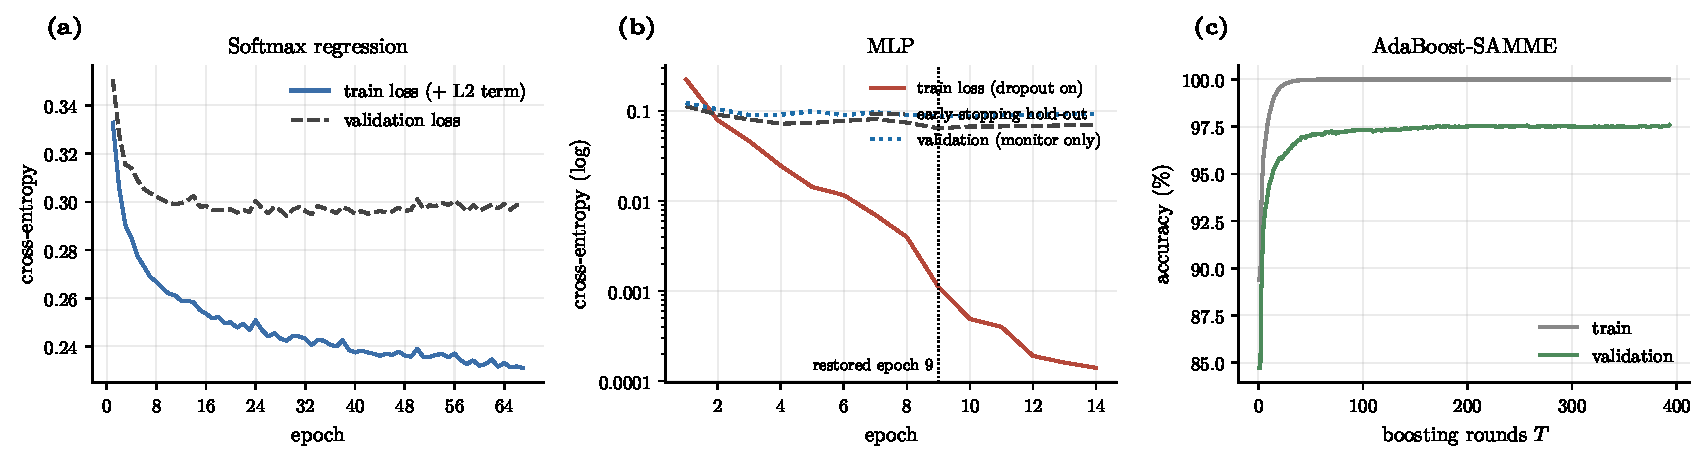
\includegraphics[width=\textwidth]{../results/figures/learning_curves.pdf}
\caption{(a) softmax: loss train có cộng thành phần $\ell_2$ (bằng 0 ở cấu hình được chọn) và loss validation theo epoch. (b) MLP: loss train (có dropout nếu bật), loss trên tập giữ lại để dừng sớm và loss validation chỉ để theo dõi; epoch tốt nhất được khôi phục. (c) AdaBoost: độ chính xác theo số vòng boosting.}
\label{fig:curves}
\end{figure}
